\documentclass[12pt]{l4dc2021}
% common symbols
\newcommand{\Real}{\mathbb{R}}
\newcommand{\rank}{\operatorname{rank}}
\newcommand{\hank}{\mathcal{H}}

% delimited expressions
\newcommand{\braces}[1]{\left\lbrace{#1}\right\rbrace}
\newcommand{\bracks}[1]{\left\lbrack{#1}\right\rbrack}
\newcommand{\angles}[1]{\left\langle{#1}\right\rangle}
\newcommand{\verts}[1]{\left\vert{#1}\right\vert}
\newcommand{\Verts}[1]{\left\Vert{#1}\right\Vert}
\newcommand{\parens}[1]{\left({#1}\right)}

% expectation
\DeclareMathOperator*{\expectationSymbol}{\mathbb{E}}
\newcommand{\expectation}[2]{\expectationSymbol_{#1}\bracks{#2}}


% The following packages will be automatically loaded:
% amsmath, amssymb, natbib, graphicx, url, algorithm2e

\title[System Identification using Low-rank Matrix Recovery]
{CIS 618 Project Report: System Identification using Low-rank Matrix Recovery}
\usepackage{times}
\usepackage{graphicx}
\graphicspath{{./figs/}}
% Use \Name{Author Name} to specify the name.
% If the surname contains spaces, enclose the surname
% in braces, e.g. \Name{John {Smith Jones}} similarly
% if the name has a "von" part, e.g \Name{Jane {de Winter}}.
% If the first letter in the forenames is a diacritic
% enclose the diacritic in braces, e.g. \Name{{\'E}louise Smith}

% Two authors with the same address
% \coltauthor{\Name{Author Name1} \Email{abc@sample.com}\and
%  \Name{Author Name2} \Email{xyz@sample.com}\\
%  \addr Address}

% Three or more authors with the same address:
% \coltauthor{\Name{Author Name1} \Email{an1@sample.com}\\
%  \Name{Author Name2} \Email{an2@sample.com}\\
%  \Name{Author Name3} \Email{an3@sample.com}\\
%  \addr Address}

% Authors with different addresses:
\author{%
 \Name{Steve Hsu} \Email{stevehsu@seas.upenn.edu}\\
 \addr University of Pennsylvania
}

\begin{document}

\maketitle

\begin{abstract}%
  We explore the circumstances under which
  low-rank matrix recovery gives good estimates
  of the Markov parameters of a partially observed LTI system.
  We build on previous results that do not use low-rank matrix recovery
  and on results that use low-rank matrix recovery
  in systems without process noise.
\end{abstract}

\begin{keywords}%
  rank minimization, system identification, convex optimization
\end{keywords}

\section{Problem Formulation}

We focus on the system identification problem
described by \cite{oymak2019singletraj}.
Consider a linear system with
state space $\Real^n$ where $n$ is unknown,
input space $\Real^p$,
and observation space $\Real^m$,
and dynamics
\begin{align*}
x_{t+1} &= A x_t + B u_t + w_t \\
y_t &= C x_t + D u_t + z_t \\
w_t &\sim \mathcal N (0, \sigma_w I_n) \\
z_t &\sim \mathcal N (0, \sigma_z I_m)
\end{align*}
where the system parameters $A$, $B$, $C$, and $D$
are matrices with the appropriate dimensions
and the $w_t$ and $z_t$ are independent.
Suppose we want to learn the system parameters
(up to a similarity transform)
by running a single-trajectory experiment.

\section{Related Works}

\cite{oymak2019singletraj} show
that for suitably chosen $K$, a good estimate of the Markov parameters
\begin{align*}
G &= \begin{bmatrix} D & G_0 & G_1 & \cdots & G_{K-2} \end{bmatrix} \\
&= \begin{bmatrix} D & CB & CAB & \cdots & C A^{K-2} B \end{bmatrix}
\end{align*}
can be used to obtain good estimates of the system parameters
up to a similarity transform.
We can therefore focus on estimating the Markov parameters,
and it will follow from this result
that we can then obtain a good system realization.

\cite{oymak2019singletraj} also give
an algorithm that estimates the Markov parameters in the single-trajectory setting,
and they show that the estimated Markov parameters
converge to the true Markov parameters when $\rho(A) < 1$.
\cite{simchowitz2019parametric} modify
the algorithm by \cite{oymak2019singletraj},
and they show that the estimated Markov parameters produced by the modified algorithm
converge to the true Markov parameters when $\rho(A) \le 1$,
even in the presence of adversarial noise.

\cite{recht2010lowrank} show that,
in the episodic setting and in the absence of noise,
if the control inputs $u_t^n \sim \mathcal N (0, \sigma_u I_m)$
are independent,
then the solution to
\begin{align*}
  \minimize &\Verts{\mathcal H (\hat G)}_\star \\
  \subject & \hat G \bar u^n = y^n_T \text{ for all $n$}
\end{align*}
minimizes the rank of $\mathcal H(\hat G)$ and therefore
produces a minimal realization of the system,
where
$\mathcal H(G)$ is called the Hankel matrix of $G$,
\[
  \mathcal H(G) = \begin{bmatrix}
    D & G_0 & \cdots & G_{T_2-1} \\
    G_0 & G_1 & \cdots & G_{T_2} \\
    \vdots & \vdots & \ddots & \vdots \\
    G_{T_1-1} & G_{T_1} & \cdots & G_{T_1 + T_2 - 1}
  \end{bmatrix},
  \qquad
  \bar u ^n = \begin{bmatrix} u^n_{T-1} \\ u^n_{T-1} \\ \vdots \\ u^n_0 \end{bmatrix},
\]
and $T = T_1 + T_2 + 1$ is the length of each episode.

\cite{fazel2013hankel} give algorithms for Schatten 1-norm minimization
on structured matrices, such as Hankel matrices,
and they allow for noise in the
constraints of the rank minimization problem.
They also provide Matlab implementations of their algorithms
and provide experimental results in the single-trajectory setting
with measurement noise (i.e.\ $\sigma_z \ne 0$)
and no process noise (i.e.\ $\sigma_w = 0$).

\begin{frame}
\frametitle{Agenda}
\begin{itemize}
\item Problem setup
\item \textbf{Least squares}
\item Low-rank matrix recovery
\item Conclusion
\end{itemize}
\end{frame}

\begin{frame}
\frametitle{Ordinary least squares}
\[ y_t = G \overline{u}_t + F \overline{w}_t + z_t + C A^{T-1} x_{t-T+1} \]

ignoring $C A^{T-1} x_{t-T+1}$ for now, take
\[ \hat G = \arg\min_G \Verts{G \overline{U} - Y}_F^2 \]

taken from
``Non-asymptotic identification of LTI systems from a single trajectory''
by Oymak and Ozay, 2019
\end{frame}

\begin{frame}
\frametitle{Prefiltered least squares}
\[ y_t = G \overline{u}_t + F \overline{w}_t + z_t + C A^{T-1} x_{t-T+1} \]
can we kill off the $C A^{T-1} x_{t-T+1}$ term?

idea: subtract off the component of $y_t$ correlated with $y_{t-T}$, $y_{t-T-1}$, etc.

\begin{align*}
\phi &= \arg\min_\varphi \Verts{\varphi K - Y}_F^2 + \mu \Verts{\varphi}_F^2 \\
\hat G &= \arg\min_G \Verts{G \overline{U} - (Y - \phi K)}_F^2
\end{align*}
where $K$ is a matrix whose $t$th column is
$[y_{t-T}^\top, y_{t-2T}^\top, \ldots, y_{t-LT}^\top]^\top$
for some fixed constant $L$

taken from
``Learning linear dynamical linear systems with semi-parametric least squares''
by Simchowitz, Boczar, and Recht, 2019
\end{frame}

\begin{frame}
\frametitle{Simple averaging}
fact from Oymak and Ozay:
\[
\expectation{}{\frac{1}{\sigma_u^2} y_t u_{t-k}^\top} = \begin{cases}
D & \text{if } k = 0 \\
C A^{k-1} B & \text{if } k \ge 1 \\
\end{cases}
\]

we can therefore also estimate $G$ using a simple average:
\[ \hat G = \frac{1}{N \sigma_u^2} Y \overline{U}^\top \]
where $N + T - 1$ is the length of the trajectory
\end{frame}

\begin{frame}
\begin{figure}
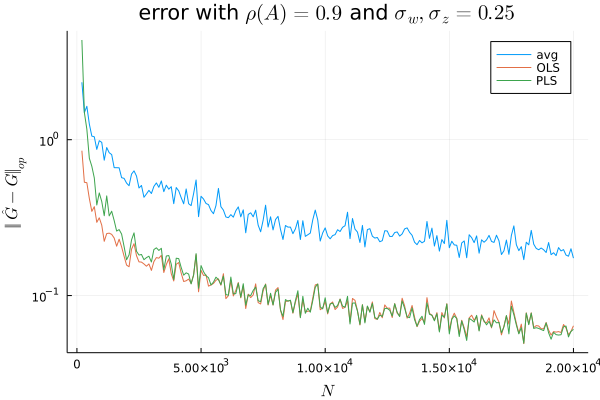
\includegraphics[scale=0.6]{rho_small}
\end{figure}
\end{frame}

\begin{frame}
\begin{figure}
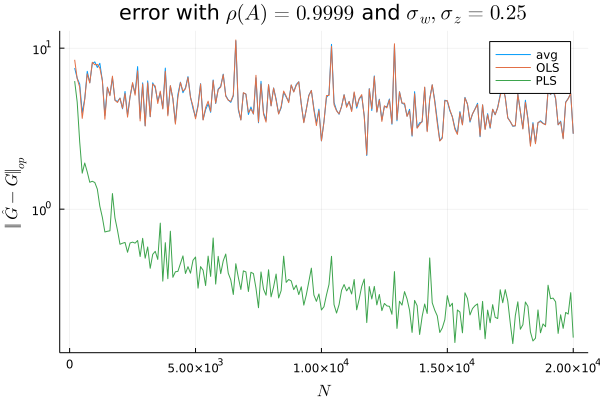
\includegraphics[scale=0.6]{rho_1me}
\end{figure}
\end{frame}

\begin{frame}
\begin{figure}
\includegraphics[scale=0.6]{baseline_stability}
\end{figure}
\end{frame}

\begin{frame}
\frametitle{Agenda}
\begin{itemize}
\item Problem setup
\item Least squares
\item \textbf{Low-rank matrix recovery}
\item Conclusion
\end{itemize}
\end{frame}

\begin{frame}
\frametitle{Motivation}
Ho-Kalman involves forming the Hankel matrix $\hank(\hat G)$, where
\[
  \hank(G) = \begin{bmatrix}
    D & G_0 & \cdots & G_{T_2-1} \\
    G_0 & G_1 & \cdots & G_{T_2} \\
    \vdots & \vdots & \ddots & \vdots \\
    G_{T_1-1} & G_{T_1} & \cdots & G_{T_1 + T_2 - 1}
  \end{bmatrix}
\]
taking its SVD, and zeroing out all but the top $n$ singular values
in order to produce a system realization with order $n$
(i.e. $\hat A$ is $n \times n$)

when producing our estimate $\hat G$,
we might want to constrain it to have rank at most $n$ like this:
\[
\hat G = \arg\min_G \Verts{G \overline{U} - Y}_F^2 \quad
\text{such that} \quad \rank\parens{\hank(G)} \le n
\]
\end{frame}

\begin{frame}
\frametitle{Schatten 1-norm minimization}
\[
\hat G = \arg\min_G \Verts{G \overline{U} - Y}_F^2 \quad
\text{such that} \quad \rank\parens{\hank(G)} \le n
\]

\[
\frac{1}{2} \begin{bmatrix} 1 & 0 \\ 0 & 0 \end{bmatrix}
+ \frac{1}{2} \begin{bmatrix} 0 & 0 \\ 0 & 1 \end{bmatrix}
= \begin{bmatrix} 1/2 & 0 \\ 0 & 1/2 \end{bmatrix}
\]
the rank function is not convex, so we use the Schatten 1-norm as a heuristic:
\[
\hat G = \arg\min_G \frac{1}{2} \Verts{G \overline{U} - Y}_F^2 + \mu \Verts{\hank(G)}_\star
\]

I implemented algorithms for this problem presented in
``Hankel matrix rank minimization
with applications to system identification and realization''
by Fazel, Pong, Sun, and Tseng, 2013
\end{frame}

\begin{frame}
\begin{figure}
\includegraphics[scale=0.6]{unfiltered_rho_small}
\end{figure}
\end{frame}

\begin{frame}
\begin{figure}
\includegraphics[scale=0.6]{unfiltered_rho_1me}
\end{figure}
\end{frame}

\begin{frame}
\frametitle{Schatten 1-norm minimization with prefiltering}
I tried doing the same thing with prefiltered least squares:
\begin{align*}
\phi &= \arg\min_\varphi \Verts{\varphi K - Y}_F^2 + \mu_{\text{PF}} \Verts{\varphi}_F^2 \\
\hat G &= \arg\min_G \frac{1}{2} \Verts{G \overline{U} - (Y - \phi K)}_F^2 + \mu \Verts{\hank(G)}_\star
\end{align*}
\end{frame}

\begin{frame}
\begin{figure}
\includegraphics[scale=0.6]{prefiltered_rho_1me}
\end{figure}
\end{frame}

\begin{frame}
\frametitle{Agenda}
\begin{itemize}
\item Problem setup
\item Least squares
\item Low-rank matrix recovery
\item \textbf{Conclusion}
\end{itemize}
\end{frame}

\begin{frame}
\frametitle{Conclusion}
minimizing the rank of $\hank(\hat G)$
didn't produce better estimates $\hat G$

Fazel et al show that Hankel matrix rank minimization
can be used to eliminate observation noise:
the solution to
\[ \arg\min _{\hat Y} \frac{1}{2} \Verts{\hat Y - Y}_F^2 + \mu \Verts{\hank(Y) U^\bot}_\star \]
gives a good estimate of $y_t - z_t = C x_t + D u_t$

maybe applying Hankel matrix rank minimization elsewhere
will give better estimates of system parameters than least squares
\end{frame}


% Acknowledgments---Will not appear in anonymized version
%\acks{We thank a bunch of people.}

\bibliography{references.bib}

\end{document}
